\documentclass[times]{elsarticle}
\usepackage[margin=2cm]{geometry}
%\documentclass[]{elsarticle}
\usepackage[labelfont=bf,justification=raggedright]{caption}
\captionsetup[figure]{name=Fig. ,labelsep=period,singlelinecheck=true,skip=5pt}
\captionsetup[table]{labelsep=newline,font=footnotesize,singlelinecheck=false,skip=5pt}
%\documentclass[final,5p,times,twocolumn]{elsarticle}
%\setlength{\mathindent}{3cm}
%Function format
\usepackage{lineno,hyperref}
\modulolinenumbers[5]
	 
	\journal{Computational Materaials Science}
	
	%%%%%%%%%%%%%%%%%%%%%%%
	%% Elsevier bibliography styles
	%%%%%%%%%%%%%%%%%%%%%%%
	%% To change the style, put a % in front of the second line of the current style and
	%% remove the % from the second line of the style you would like to use.
	%%%%%%%%%%%%%%%%%%%%%%%
	
	%% Numbered
	%\bibliographystyle{model1-num-names}

	%% Numbered without titles2
	%\bibliographystyle{model1a-num-names}
	
	%% Harvard
\bibliographystyle{elsarticle-num.bst}
\modulolinenumbers[5]
\journal{Materials and Design}
%%%%%%%%%%%%%%%%%%%%%%%
\begin{document}
\begin{frontmatter}
\title{Effect of Nanovoid on Fracture Process of Two-Phase $\alpha$($\rm TiAl$)+$\gamma$($\rm Ti_3Al$) Alloy}
%\tnotetext[mytitlenote]{*** \href{http: //www.ctan.org/tex-archive/macros/latex/contrib/elsarticle}{CTAN}.}
%% Group authors per affiliation:
%\author{Maomao Wang\fnref{myfootnote}}

\address[mymainaddress]{School of Mechanical and Electronical Engineering, Lanzhou University of Technology. Lanzhou 730050, China}
\begin{abstract}
Fracture processes of nanocrystalline metallic materia is affected by dislocation, nanovoid and other defects. Existing studies of defect evolution in titanium-aluminium alloy cover the case that voids located in single crystals, inside grain in poly crystals and at the grain boundaries.Molecular dynamics simulation was performed to study the evolution of a spherical nanovoid in $\alpha$+$\gamma$ two-phase titanium-aluminium alloy under uniaxial tension. The results show that voids located at the $\alpha$/$\gamma$ phase boundary have significant detract to strength of Ti-Al polycrystalline.
\end{abstract}

\begin{keyword}
$\alpha$+$\gamma$ two phase TiAl alloy; void; molecular dynamics
\end{keyword}

\end{frontmatter}
\linenumbers

\section{Introduction}
\paragraph{Material}
TiAl alloy has been used as structural material in aviation industry because its inherent advantages such as low density and self-diffusion rates, high elastic module and high strength \cite{vu2013}.However, single phase $\gamma-\rm TiAl$ generally brittle at room temperatures and this limits their use in many other fields.Two-phase titanium aluminum alloys with proper phase distribution and grain size exhibit better mechanical performance compared with monolithic constituents $\gamma$(TiAl) and $\gamma$($\rm Ti_3Al$) alloy \cite{}.

\paragraph{Void}
Two phase titanium aluminide alloys exhibit a much better mechanical performance than their monolithic constituents $\gamma$(TiAl) and $\alpha_2$ (Ti3Al), provided that the phase distribution and grain size are suitably controlled. Two-phase titantium aliuminde alloys with proper phase distribution and grain size exhibit better mechanicalperformance compared with monolithicconstituents gamma and alpha[].
Brittle fracture in TiAl alloy strongly affects the safety of fracture of structure like turbo of aircraft engine andcombustion generator.

The failure modes of materials have significant influence on the design of material properties in materials science. Rapture failure at the macroscopic scale can be attributed to nucleation, growth and propagation of cracks, but at the microscopic scale cracks are initially easily formed at defects in the casting process, such as voids and inclusions [1].These defects are known to play a fundamental role in the deformation of the material. Nucleation, growth and coalescence of voids are deemed as the primary mechanism of ductile material fracture, in which void growth is particularly important. Therefore, it is necessary to study the deformation response of porous materials with the consideration of microstructure evolution.


Two phase titanium aluminide alloys exhibit a much better mechanical performance than their monolithic constituents $\gamma$(TiAl) and $\alpha_2$ (Ti3Al), provided that the phase distribution and grain size are suitably controlled. Two-phase titantium aliuminde alloys with proper phase distribution and grain size exhibit better mechanicalperformance compared with monolithicconstituents gamma and alpha[].
Brittle fracture in TiAl alloy strongly affects the safety of fracture of structure like turbo of aircraft engine andcombustion generator[].Defects such as dislocation, void and segregation plays an significant role in the process of fracture[].In order to understanding the mechanism of brittle fracture, multi-scale methods from micro to marco scale have been applied to investigate the behavior of fracture. It's necessary to carefully examine the revolution of defects and its influence on the fracture process at atomic scale.
A previous study on void growth in gamma-TiAl single crystal has reveals that void with high volume fraction detracts incipient yield strength [].
Molecular dynamics(MD method has been use to investigate the evolution of void in materials in nano-
scale[].
The fracture mechanisms in the duplex micro-structure are plasticity-induced grain boundary de- cohesion
and cleavage, while those in the lamellar microstructure are interface delamination and crack- ing across the
lamellae[].

\section{Molecular Dynamics Simulation }

\subsection{Atomic Potential}
The interaction of particle in the material is determined by interatomic potential. Many reported examples of crack propagation in metal materials were performed with embedded atomic method due to is better accuracy in metal lattice compare with F-S and L/J \cite{}. The embedded atom method (MEAM) potential developed by Zope and Mishin by \cite{} was used in the study. The simulation is submitted by MD simulations with the Large-scale Atomic/Molecular Massively Parallel Simulator (LAMMPS) open-source code \cite{}. We performed constant-pressure and constant-temperature (NPT) molecular dynamics simulation.

\begin{equation} \label{eq:eam} 
	E= \displaystyle\sum
\end{equation}

\subsection{Model Creation of Crystalline}
$\gamma $ TiAl has a fcc-centered tetragonal with an $L1_0$ structure \cite{}, and $\alpha TiAl$ is hcp structure, the structure of the two initial cells are shown in Fig.\cite{}, and the constructing parameters are givin by Table.\cite{}. The simulation cells of two phase polycrystalline with an initially spherical void at different position are shown in figure \cite{}. Periodic boundary conditions (PBC)are applied along all three directions, that makes poly crystal with periodic nanovoid structures. The initial dimension of simulation cell is  $L_x = $ nm, $L_y = $ nm, $L_z = $ nm, and each model contains about 4.6 million atoms. The grain orientation and size were randomly created with Voronoi method with code ATOMSK \cite{}, and resulting in the arbitrary shape and orientation of the grains. Only one spherical void defect was placed intragranularlly or intergranularlly within each simulation model void within each simulation model. The intragranular spherical void was located in grain interior of the largest grain of the simulation model, as shown in Fig. \cite{}. The intergranular spherical void was at the center of the simulation cell, as shown in Fig. \cite{}.



\begin{table}[h]
\centering
\caption{Parameters of  nanocrystalline}

\begin{tabular}{l c c l}
\hline
			Phase			& Space group		& Designation		& Parameters \\
			\hline
			$\alpha_2$		& $\rm P6_3/mmc$ 	& $\rm 0_{19}$ 		& $a$ = 0.5765 \\
							&					&					& $c$ = 0.46833 \\
			$\gamma$		& $\rm tP4$ 		& $\rm L1_0$		& $a$ = 0.3997 \\
			 				&					&					& $c$ = 0.4062 \\			
			\hline
\end{tabular}
	\label{tab:lattice_parameter}
\end{table}
 
\subsection{Analysis method}
\paragraph{CSP}
The centrosymmetry parameter is defined as follow:
\begin{equation} \label{eq:csp} 
	P = \displaystyle\sum_{i=1}^{6}|\vec{R_i}+\vec{R_{i+6}}|^2
\end{equation}

where $\vec{R_i}$ and $\vec{R_{i+6}}$ are the vectors corresponding to the six pairs of opposite nearest neighbors in the fcc lattice. The centrosymmetry parameter(CSP) is zero for atoms in a perfect lattice. In other words, if the lattice is distorted the value of P will not be zero. Instead, the parameter will have a value within the range corresponding to a particular defect. By removing all the perfect and surface atoms within the bulk, the existence of dislocation atoms become visible.
	
\paragraph{Virial Stress}
The atomic stress is calculated using the virial definition :
$$\sigma_t(i)=-$$
$$\sigma_t(i)= $$
 
\section{Results and Discussion}

\subsection{Deformation Mechanisms in Two-Phase Alloys}
Deformation phenomena in TiAl alloys have been widely studied in order to overcome the problems associated with the limited ductility and damage tolerance. The literature data covers a wide range of parameters such as alloy composition, microstructure and deformation temperature. Much of the work has been performed on single phase $\gamma$ alloys and PST crystals. However, the following discussion concentrates on deformation phenomena that rely on the elastoplastic codeformation of the $\gamma$ and $\gamma_2$ phases and on the particular point defect situation occurring in two - phase alloys. Due to this effect ( $\alpha_2$ + $\gamma$ ) alloys exhibit some remarkable properties that are unlike those of either constituent.

\subsection{Fracture Process}
\paragraph{initiation of crack}
\paragraph{fracture process}
The existence of void detract the strength, and the void inside $\alpha$ phase grain have most significant  impact on the strength, however the void on the grain boundary have little impact on incipient strength of the material. Detailed observation of specimen with void inside the grain is shown in Figure \cite{}.
1.In many cases the orientation of slip slip is changed because the crystallographically available slip and directions are not continuous across the interface. This may significantly reduce the Schmid factor and thus impede slip transfer. At the $\gamma/\gamma$ interfaces the orientation of the slip plan could change through a relevantly large angle of about 90 degree. Reorientation of slip is always required at the $\alpha_{2}/\gamma$ interface; the smallest angle between the corresponding slip planes ${1 1 1 }_{\gamma}$ and ${ 1 0 -1 0}_{\alpha_2}$ is about 19 degree \cite{}.

The core of  a dislocation intersecting an interface often needs to be transformed. For example, an ordinary 1/2<110] dislocation gliding in one $\gamma$ grain has to be converted in to a <101] super dislocation with the double Burgers vector gliding in an adjacent $\gamma$ grain. At the $\alpha/\gamma$ interface the dislocations existing in the $D0_{19}$ structure have to be transformed into dislocations consistent with the $L1_0$structure. These core transformations are associated with a change of the dislocation line energy because the lengths of the Burgers vectors and the shear module are different.
 
Dislocations crossing semi-coherent boundaries have to intersect the misfit dislocations, a process that involves elastic interaction, jog formation and the incorporation of gliding dislocations into the mismatch structure of the interface.When the slip is forced to cross $\alpha_2$ lamella, pyramidal slip of the $\alpha_2$ phase is required, which needs an extremely high shear stress.


%\subsection{Fracture Process with Integranular Void }

%\subsection{Fracture Process with Intergranular Void }

\subsection{Evolution of spherical void in the simulation with intragranular spherical voids}
A step, of the width of a burgers vector, will be generated at both sidesof a crystal along teh direction of teh burgers vector after dislocation traversing teh entire crystal, as is shown in \ref{fig:}. A small tep will be formed at spherical void surface toward teh void interiorafter dislocation absorptionat sphericalvoid surfaces, as is shown in \ref{fig:}. If a great number of dislocation slip along their respective systemstowards teh spherical nanovoid in all directions, and are absorbed at spherical void surfaces, the spherical nanovoid will eventually shrink from teh dash circle to

\begin{figure}
	\centering
	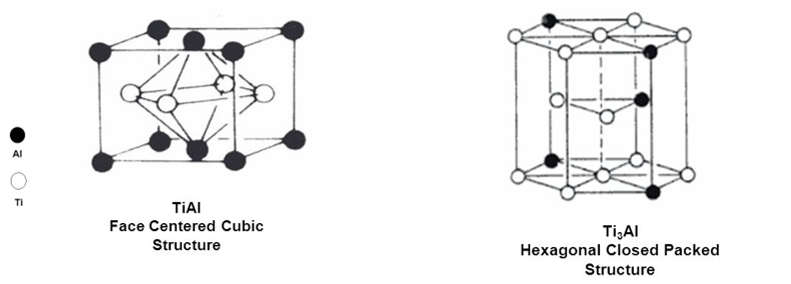
\includegraphics[width=0.7\linewidth]{img/cell}
	\caption{unit cell}
	\label{fig:unit_cell}
\end{figure}

\begin{figure}
	\centering
	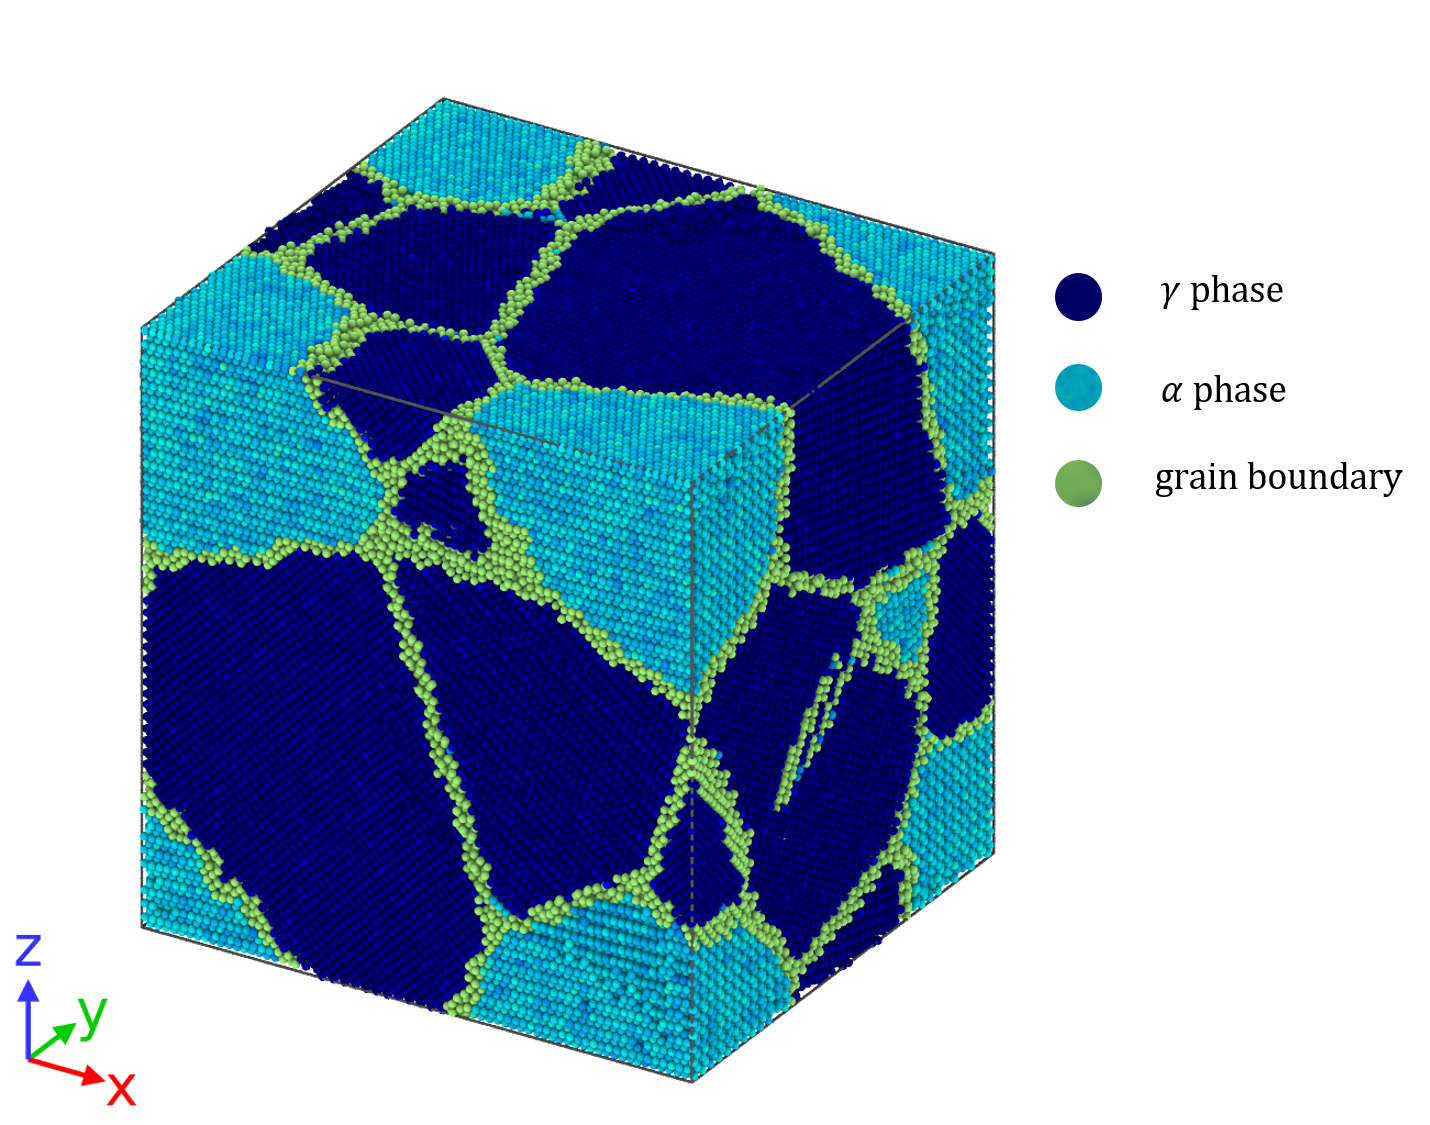
\includegraphics[width=0.7\linewidth]{img/pf_model_labeled}
	\caption{Simulation box}
	\label{fig:simulation_box}
\end{figure}


\begin{figure}
	\centering
	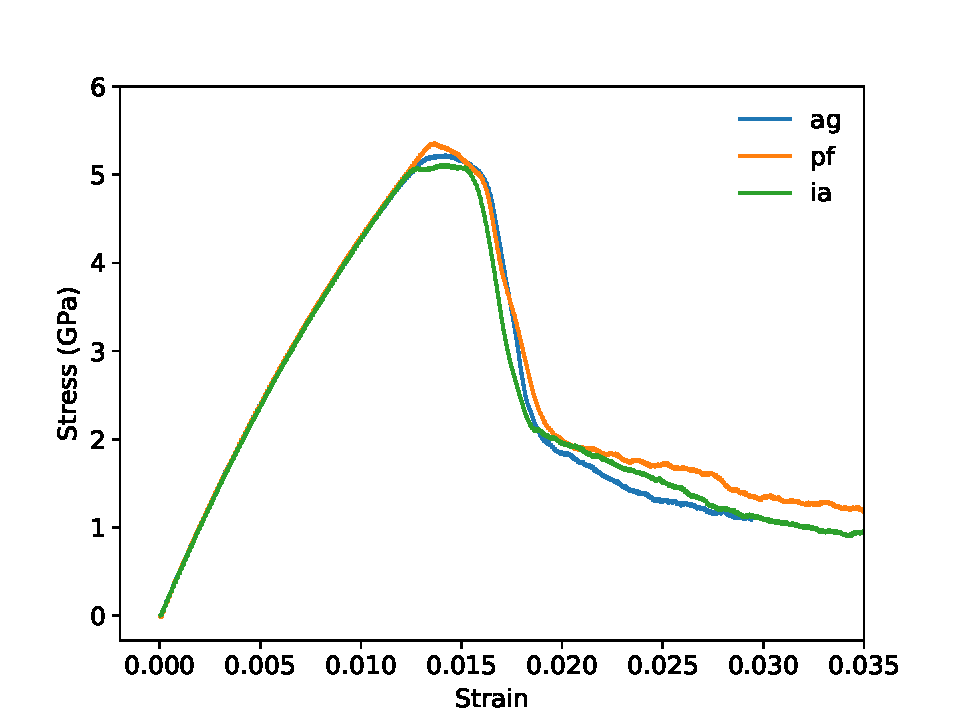
\includegraphics[width=0.7\linewidth]{img/allline}
	\caption{Fracture process of specimen with void in $\alpha$ phase}
	\label{fig:all_line}
\end{figure}

%\subsection{The influence of void on strength of TiAl alloy}
\begin{figure}
	\centering
	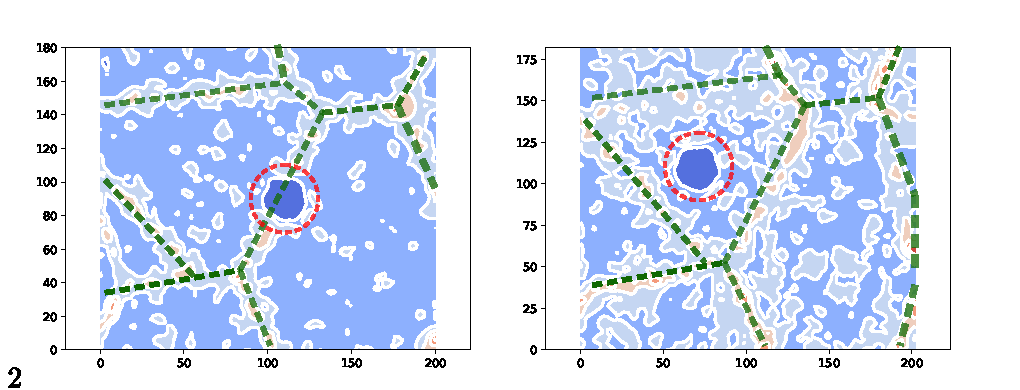
\includegraphics[width=0.7\linewidth]{img/frame2}
	\caption{stress-$\sigma$=0}
	\label{fig:all_line}
\end{figure}

\begin{figure}
	\centering
	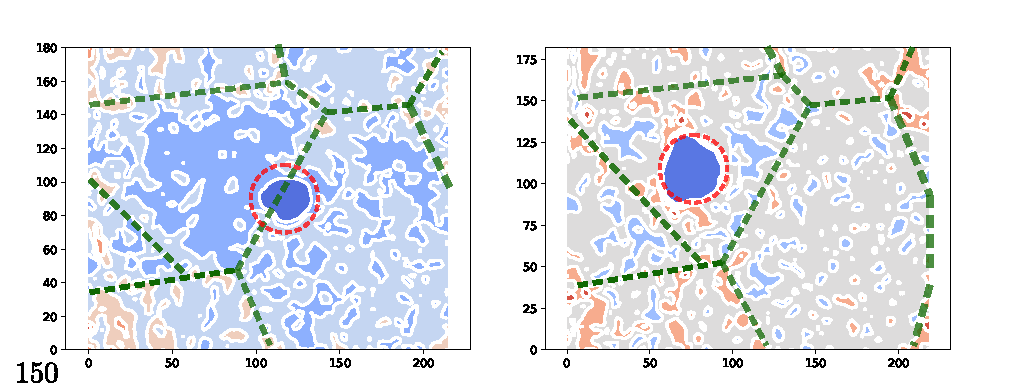
\includegraphics[width=0.7\linewidth]{img/frame150}
	\caption{stress-$\sigma$=0.15}
	\label{fig:all_line}
\end{figure}

\begin{figure}
	\centering
	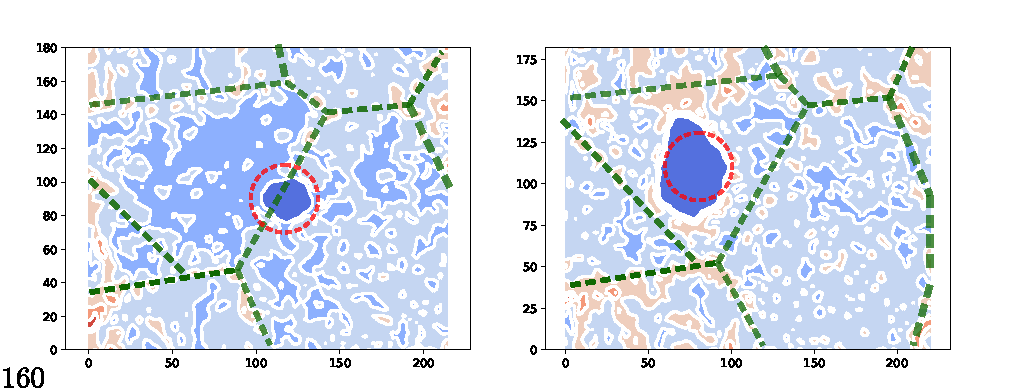
\includegraphics[width=0.7\linewidth]{img/frame160}
	\caption{stress-$\sigma$=0.16}
	\label{fig:all_line}
\end{figure}

\begin{figure}
	\centering
	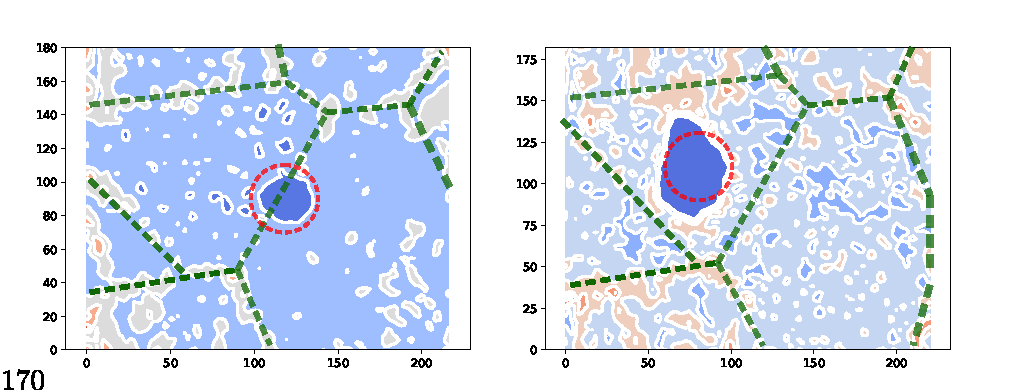
\includegraphics[width=0.7\linewidth]{img/frame170}
	\caption{stress-$\sigma$=0.17}
	\label{fig:all_line}
\end{figure}


\begin{figure}
	\centering
	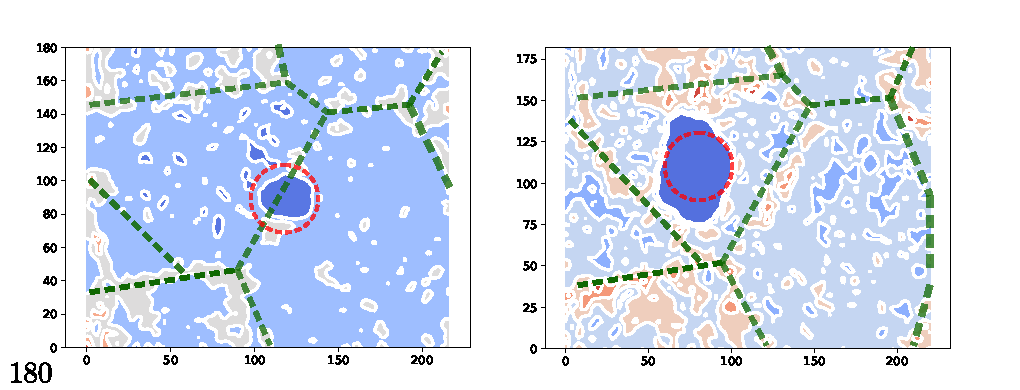
\includegraphics[width=0.7\linewidth]{img/frame180}
	\caption{stress-$\sigma$=0.18}
	\label{fig:all_line}
\end{figure}

\begin{figure}
	\centering
 	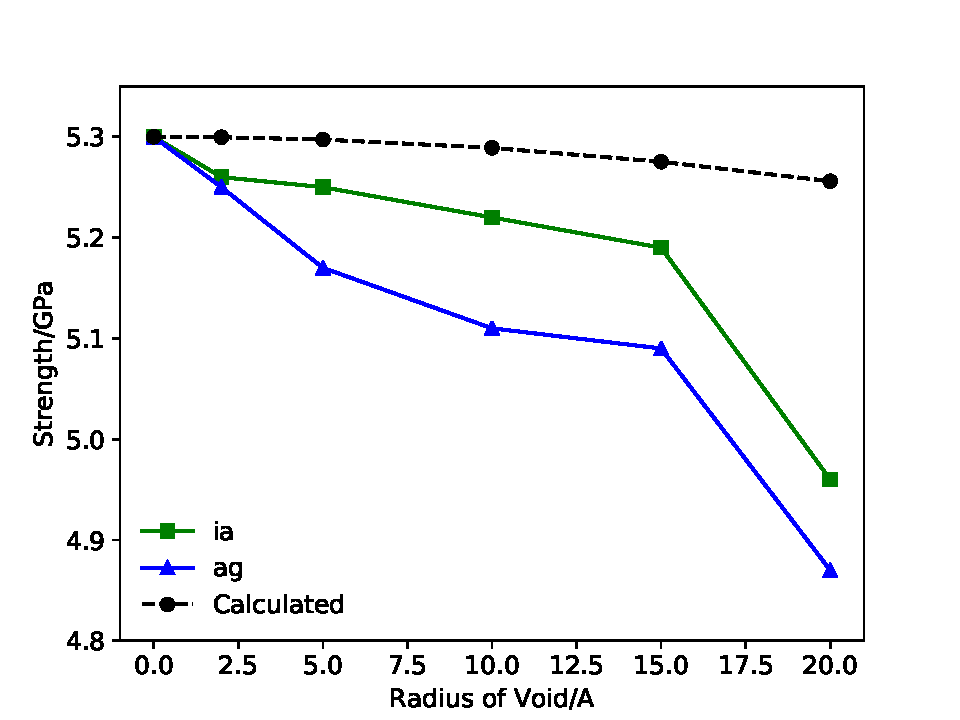
\includegraphics[width=0.7\linewidth]{img/effect_of_vol}
	\caption{}
	\label{fig:voleff}
\end{figure}

\subsection{Effect of Void Size}
\paragraph{size}
Voids with different size: 2A, 5A, 10A, 15A were placed into the model respectively. It has been observed that  voids detracts the strengths of the material. The max stress stress of the simulation cell decreases as the volume of voids are lareger. From Fig \ref{fig:voleff}, there is a critical value of void radius about 15A, the void greater than 15A cause serious detraction of strength of material. 
Engineering stress is calculated
$$ \sigma = S/A$$
The rate of decrease of loading area are smaller comparing with the detraction of strength, so it can be assumed that the yield yield behaviour and strength is much more related with local behaviour of grain boundaries and void.

Grain and phase boundaris are obstancles to deformation process, thus the stability of boundaries have great impact on the strength of materials. Interactive between grainboundary and void determins the fracture mode of the TiAl alloy.

According to Schmid's law:
$$\tau = \sigma*m$$
where m is the Schmid factor :
$$ m = cos(\phi)cos(\lambda)$$

\paragraph{position}critical void 
The location of void affects strength of material. Comparing with the model with integranular void, the model with intergranular voids is weaker. atomic stress is calculated 

\begin{figure}
	\centering
	\includegraphics[width=1\linewidth]{"img/fracture3"}
	\caption{Fracture Process}
	\label{fig:fracture-process}
\end{figure}




\begin{figure}
	\centering
	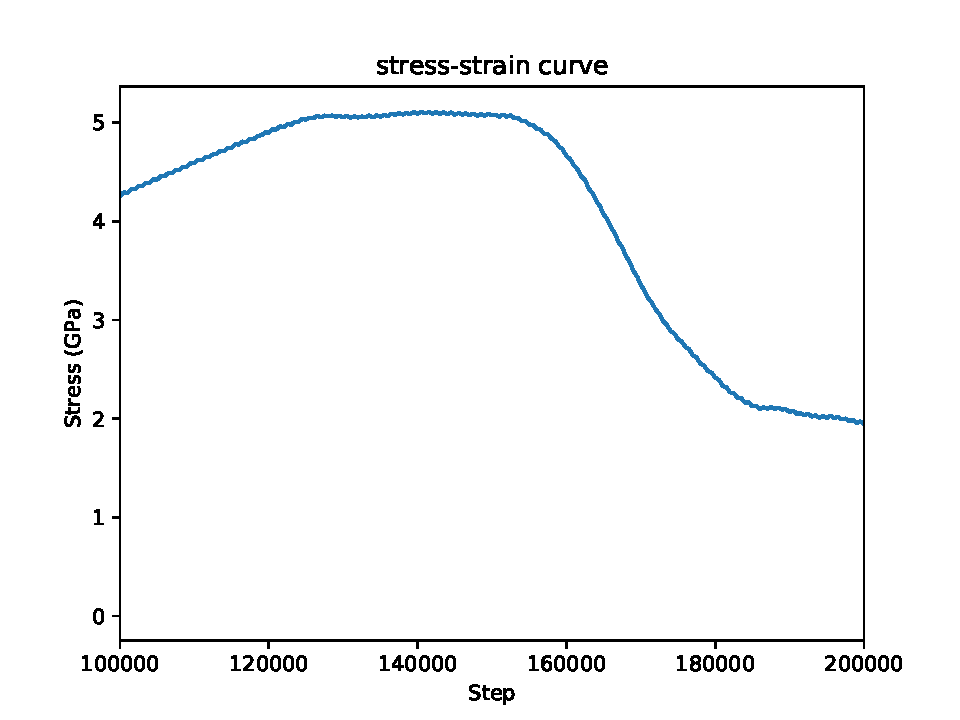
\includegraphics[width=0.7\linewidth]{img/ialine}
	\caption{stress-strain curve}
	\label{fig:ia_line}
\end{figure}

\begin{figure}
	\centering
	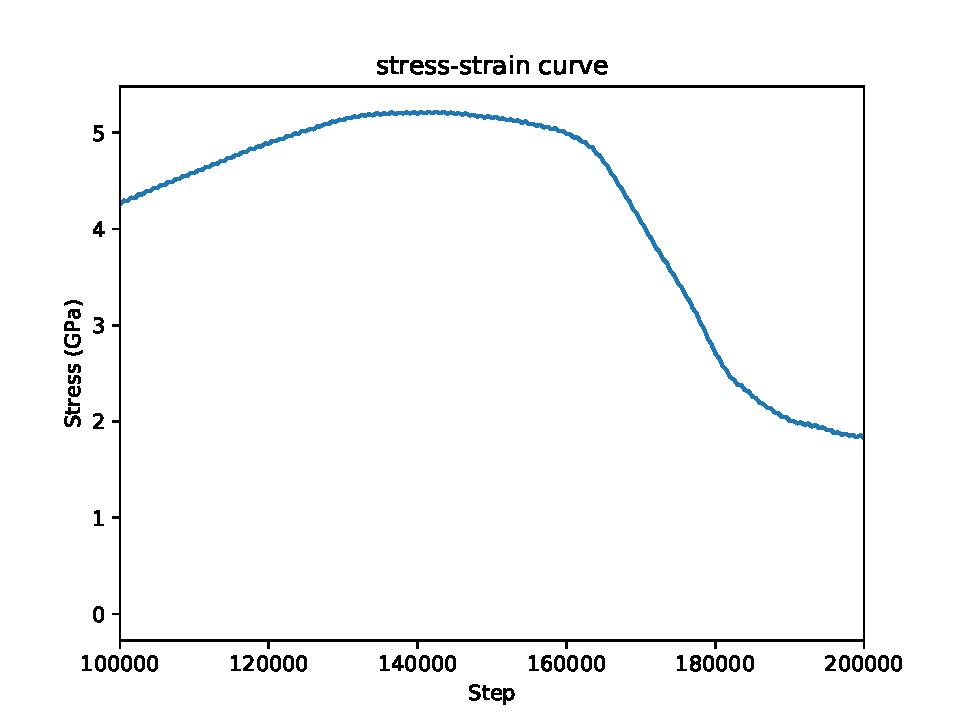
\includegraphics[width=0.7\linewidth]{img/agline}
	\caption{stress-strain curve}
	\label{fig:ag_line}
\end{figure}


\begin{figure}
	\centering
	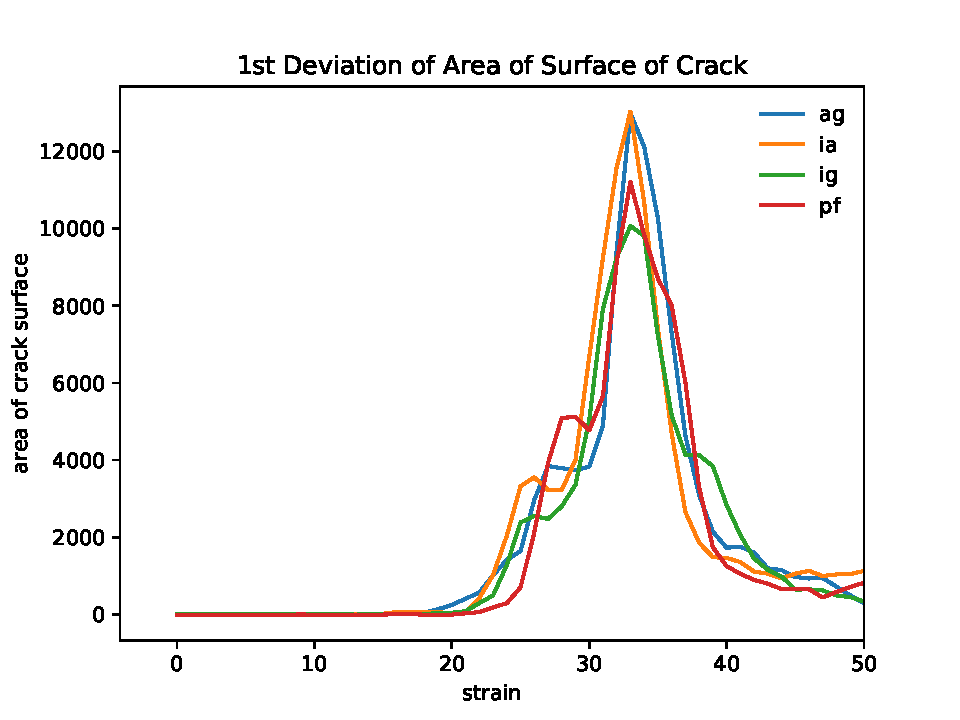
\includegraphics[width=0.7\linewidth]{img/1stdiv}
	\label{fig:surf}
	\caption{stress-strain curve}
\end{figure}


\section{Conclusion}
%\bibliographystyle{elsarticle-num.bst}

\bibliography{ref/VIOLET-ref}

\end{document}
